\chapter{Polar coordinates}
\label{ch:polar}

In this chapter,
we apply boundary tracing to the conduction--radiation problem
using the fundamental line-source solution
as the known solution to
Laplace's equation~(\ref{eq:laplace-steady-conduction}).
As in Chapter~\ref{ch:cartesian},
traced boundaries are sought along which
the radiation condition~(\ref{eq:radiation-boundary-condition})
is satisfied.
The convex portions of these traced boundaries are then used
to construct conduction--radiation domains
which admit the same line-source solution.

\section{Line-source solution}
\label{sec:polar.line}

First we establish the known solution and the appropriate scaling.

The line-source solution
to Laplace's equation~(\ref{eq:laplace-steady-conduction})
is usually encountered in electrostatics,
where it represents the potential of a line charge,
logarithmic in the cylindrical radius~$r \ideq \sqrt{x^2 + y^2}$.
In the context of steady conduction,
the only dimensionally consistent form for this is
\begin{important}{equation}
  T \ideq T_0 \log \roundbr*{\frac{r_0}{r}}
  \label{eq:line-laplace-solution}
\end{important}
for some temperature~$T_0$ and radius~$r_0$.%
\footnote{
  Whereas the power law~$T = C r^n$ is scale-invariant,
  requiring only \emph{one} constant~$C$,
  the logarithm does not possess this property;
  separate constants are required for~$T$ and for~$r$.
}
Note that the region~$r > r_0$ is unphysical,
since there the temperature is negative.

Clearly it is sensible to work in the usual polar coordinates~$(r, \phi)$
given by the transformation
\begin{align}
  x &\ideq r \cos\phi, \label{eq:x-transformation-polar} \\
  y &\ideq r \sin\phi, \label{eq:y-transformation-polar}
\end{align}
with scale factors
\begin{align}
  \scalefac[r] &\ideq 1, \label{eq:r-scale-factor-polar} \\
  \scalefac[\phi] &\ideq r. \label{eq:phi-scale-factor-polar}
\end{align}

\subsection{Scaling}
\label{sec:polar.line.scaling}

While the known solution~(\ref{eq:line-laplace-solution})
already has intrinsic temperature and length scales $T_0$ and~$r_0$,
the final scaling should also account for
the radiation boundary condition~(\ref{eq:radiation-boundary-condition}).

Let
\begin{align}
  T &\ideq \Theta \scaled{T}, \label{eq:line-temperature-scaling} \\
  r &\ideq \varrho \scaled{r}, \label{eq:line-r-scaling}
\end{align}
with~$\Theta$ and~$\varrho$ to be chosen later.
Noting that
\begin{equation}
  \del \ideq \scaleddel / \varrho,
  \label{eq:line-del-scaling}
\end{equation}
the radiation boundary condition~(\ref{eq:radiation-boundary-condition})
and the known solution~(\ref{eq:line-laplace-solution})
become
\begin{align}
  \normalvec \dotp \scaleddel \scaled{T}
    &= -\group{c \varrho \Theta^3} \scaled{T}^4,
    \label{eq:line-scaled-radiation-boundary-condition-with-groups}
    \\[\tallspace]
  \scaled{T}
    &\ideq
      \group{\frac{T_0}{\Theta}}
      \log \roundbr*{\frac{\group{r_0 / \varrho}}{\scaled{r}}}.
    \label{eq:line-scaled-laplace-solution-with-groups}
\end{align}
There are three dimensionless groups
but only two free scales~$\Theta$ and~$\varrho$,
so one of the groups cannot be eliminated.
To keep the logarithm as simple as possible,
we put
\begin{align}
  \Theta &= T_0,
    \label{eq:line-temperature-scale} \\
  \varrho &= r_0,
    \label{eq:line-length-scale}
\end{align}
and define the dimensionless group
\begin{equation}
  A = \frac{1}{c r_0 {T_0}^3}.
  \label{eq:line-dimensionless-group}
\end{equation}
Dropping \scalingmarks, the scaled boundary condition~%
  (\ref{eq:line-scaled-radiation-boundary-condition-with-groups})
and known solution~(\ref{eq:line-scaled-laplace-solution-with-groups})
become
\begin{important}{align}
  \normalvec \dotp \del T &= -\frac{T^4}{A},
    \label{eq:line-scaled-radiation-boundary-condition} \\[\tallspace]
  T &\ideq -\log r.
    \label{eq:line-scaled-laplace-solution}
\end{important}
Note that the scale factors~%
  (\ref{eq:r-scale-factor-polar}) and~(\ref{eq:phi-scale-factor-polar})
are unchanged in form by the scaling.

\section{Viable domain}
\label{sec:polar.viable}

Next we determine the geometry of the viable domain,
the region in which traced boundaries exist.

Comparing the radiation condition~%
  (\ref{eq:line-scaled-radiation-boundary-condition})
to the generic flux condition~(\ref{eq:flux-boundary-condition}),
it follows that the flux function is
\begin{align*}
  F
  &\ideq -\frac{T^4}{A} \\[\tallspace]
  &\ideq -\frac{\log^4 r}{A}.
    \yesnumber
    \label{eq:line-flux-function}
\end{align*}
The radial and azimuthal components of the gradient~$\del T$ are
\begin{align}
  P &\ideq \pder{T}{r} \ideq -\frac{1}{r},
    \label{eq:line-gradient-r-component} \\[\tallspace]
  Q &\ideq \frac{\pd T}{r \pd\phi} \ideq 0,
    \label{eq:line-gradient-phi-component}
\end{align}
and so the viability function is given by
\begin{align*}
  \Phi
  &\ideq (\del T)^2 - F^2 \\[\tallspace]
  &\ideq \frac{1}{r^2} - \frac{\log^8 r}{A^2} \\[\tallspace]
  &\ideq \frac{A^2 - \psi^2}{A^2 r^2},
    \yesnumber
    \label{eq:line-viability-function}
\end{align*}
where $\psi$~is the auxiliary function
\begin{equation}
  \psi (r) \ideq r \log^4 r.
  \label{eq:line-auxiliary-function}
\end{equation}
The viable domain is therefore the region~$\psi (r) \le A$.

\subsection{Auxiliary function properties}
\label{sec:polar.viable.psi}

\begin{figure}
  \centredfigurecontent[width=0.6\textwidth]{%
    line-auxiliary-function%
  }{
    Auxiliary function~(\ref{eq:line-auxiliary-function}).
  }
\end{figure}

Since the region~$r > 1$ is unphysical
(corresponding to negative temperature),
it is only necessary to consider~$0 \le r \le 1$.
On this interval, $\psi$~is positive
except at the endpoints~$r = 0$ and~$r = 1$, where it vanishes.
Observing that the slope
\begin{equation}
  \tder{\psi}{r} \ideq (4 + \log r) \log^3 r
  \label{eq:line-psi-r-derivative}
\end{equation}
changes sign from positive to negative
as $r$~increases through~$\ee^{-4}$,
it follows that $\psi$~has a single maximum on~$0 \le r \le 1$ at
\begin{equation}
  r = r_\nat = \ee^{-4} = 0.01832,
  \label{eq:line-r-natural}
\end{equation}
where it takes the maximal value
\begin{equation}
  \psi
  = A_\nat
  = \psi (r_\nat)
  = (4 / \ee)^4
  = 4.6888.
  \label{eq:line-a-natural}
\end{equation}
This is shown in Figure~\ref{fig:line-auxiliary-function}.

\subsection{Three regimes}
\label{sec:polar.viable.regimes}

\begin{figure}
  \newcommand*{\figurewidth}{0.85\textwidth}
  \centering
  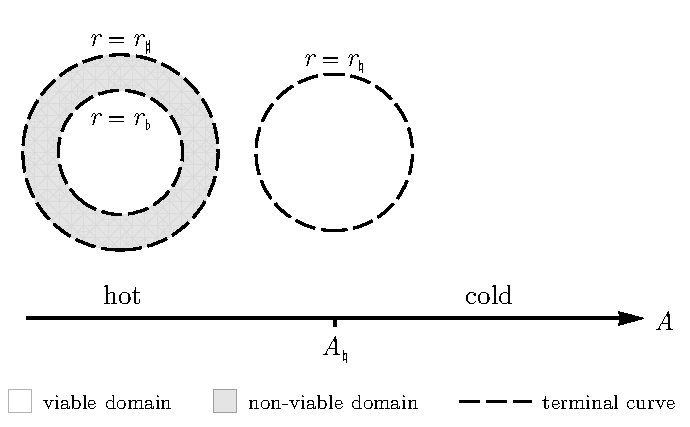
\includegraphics[width=\figurewidth]{line-viable}
  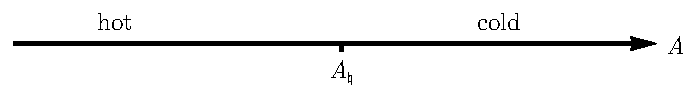
\includegraphics[width=\figurewidth]{line-viable-arrow}
  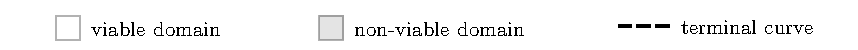
\includegraphics[width=\textwidth]{line-viable-legend}
  \caption{
    Non-viable domain~$\Phi < 0$
    for the known solution~(\ref{eq:line-scaled-laplace-solution})
    and viability function~(\ref{eq:line-viability-function}),
    as $A$~increases.
  }
  \label{fig:line-viable}
\end{figure}

The topology of the viable domain~$\psi (r) \le A$
(Figure~\ref{fig:line-viable})
will depend on whether the dimensionless group~$A$ is
less than, equal to, or greater than the critical value~$A_\nat$,
as this determines the number of roots of the equation~$\psi (r) = A$
(Figure~\ref{fig:line-critical})
corresponding to the terminal curve.
There are three cases:
\begin{enumerate}
  \item
  \label{itm:polar.regimes.hot}
    \term{Hot regime}, $A < A_\nat$:
    $\psi (r)$~is equal to~$A$ at~$r = r_\flat$ and~$r = r_\sharp$
    (both dependent on~$A$),
    with~$0 <  r_\flat < r_\nat < r_\sharp < 1$.
    The terminal curve consists of two circles,
    inner~$r = r_\flat$ and outer~$r = r_\sharp$,
    and since these are contours of the known solution~%
      (\ref{eq:line-scaled-laplace-solution}),
    the terminal curve is in fact a critical terminal curve.
    A non-viable moat~$r_\flat < r < r_\sharp$
    (in which traced boundaries do not exist)
    separates an inner viable island~$0 \le r \le r_\flat$
    from an outer viable mainland~$r \ge r_\sharp$.
  \item
    \term{Transition}, $A = A_\nat$:
    $\psi (r)$~is equal to~$A$ at~$r = r_\nat$ only,
    the two roots~$r_\flat$ and~$r_\sharp$ having merged together.
    The entire space~$0 \le r \le 1$ is now viable
    as the non-viable moat has shrunken to nothingness,
    the critical terminal curve~$r = r_\nat$
    being the only evidence of its former existence.
  \item
    \term{Cold regime}, $A > A_\nat$:
    $\psi (r)$~is never equal to~$A$.
    The entire space remains viable,
    but there is no longer any terminal curve.
\end{enumerate}

\begin{figure}
  \newcommand*{\legendoffsetheight}{0.2\textwidth}
  \centering
  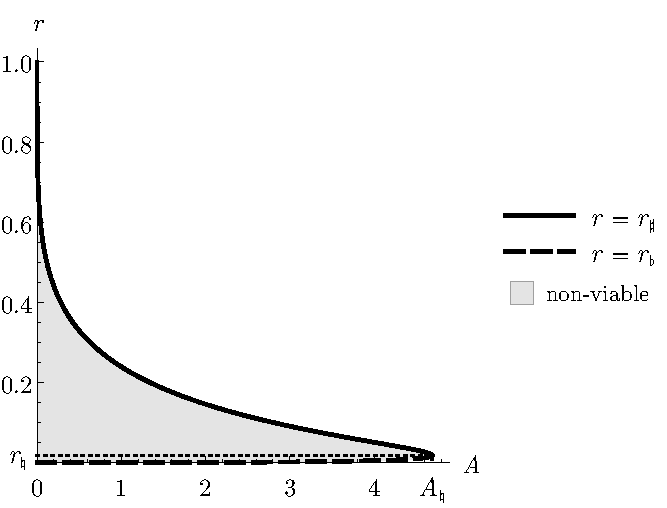
\includegraphics[width=0.5\textwidth]{line-critical}
  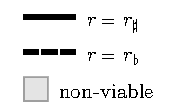
\includegraphics[
    width=0.2\textwidth,
    trim=0 {-\legendoffsetheight} 0 0
  ]{line-critical-legend}
  \caption{
    Terminal radii (roots of~$\psi (r) = A$),
    as $A$~increases.
  }
  \label{fig:line-critical}
\end{figure}

\section{Boundary tracing}
\label{sec:polar.tracing}

In this section, we write down the boundary tracing ODE
and show that the construction of convex domains
is only possible in the hot regime~$A < A_\nat$,
on the outer viable mainland~$r \ge r_\sharp$.

Using~(\ref{eq:line-flux-function})
through~(\ref{eq:line-viability-function}),
the boundary tracing ODE~(\ref{eq:tracing-ode-coordinate-parametrisation-u})
becomes
\begin{important}{equation}
  \tder{r}{\phi} = \mp \frac{\sqrt{A^2 - \psi^2}}{\log^4 r},
  \label{eq:line-tracing-ode-coordinate-parametrisation-r}
\end{important}
so that the traced boundaries are given by
\begin{important}{equation}
  \phi = \mp \int \frac{\log^4 r \td r}{\sqrt{A^2 - \psi^2}}.
  \label{eq:line-traced-boundary-integral}
\end{important}
This integral is not elementary,
and the traced boundaries must be determined numerically.
Integrating forward from various points within the viable domain,
we obtain the traced boundaries in Figure~\ref{fig:line-traced-boundaries}.

\begin{figure}
  \newcommand*{\subfigurewidth}{0.325\textwidth}
  \centering
  \begin{subfigure}{\subfigurewidth}
    \centredfigurecontent{line-traced-boundaries-hot}{Hot regime}
  \end{subfigure}
  \hfill
  \begin{subfigure}{\subfigurewidth}
    \centredfigurecontent{line-traced-boundaries-cold_hot}{Transition}
  \end{subfigure}
  \hfill
  \begin{subfigure}{\subfigurewidth}
    \centredfigurecontent{line-traced-boundaries-cold}{Cold regime}
  \end{subfigure}
  \caption{
    Traced boundaries
    obtained by integrating~(\ref{eq:line-traced-boundary-integral}).
  }
  \label{fig:line-traced-boundaries}
\end{figure}

At this point it is important to keep in mind the end goal,
which is to construct interesting domains
for which the radiation condition~%
  (\ref{eq:line-scaled-radiation-boundary-condition})
is satisfied along the boundary,
given steady conduction of the form~(\ref{eq:line-scaled-laplace-solution}).
Since the nature of the line-source singularity at~$r = 0$
is to supply heat radially at a constant power per unit length,
the only sensible configuration is for the constructed domain to
completely surround the singularity~$r = 0$ without touching it,
with the power supplied by the singularity balanced
by that lost along the outer boundary by radiation.
Therefore we seek closed curves surrounding the origin,
made by patching together the traced boundaries~%
  (\ref{eq:line-traced-boundary-integral}).

Moreover we already saw in Section~\ref{sec:cartesian.plane.domain}
that only convex domains are acceptable,
lest there be self-incident radiation which is not accounted for
by the simple radiation condition~%
  (\ref{eq:line-scaled-radiation-boundary-condition}).
The patching together of traced boundaries to form closed curves
must therefore be done diligently.

\subsection{Cold regime}
\label{sec:polar.tracing.cold}

Since the sought-after closed curve must surround the origin
and mark out a convex domain,
we may parametrise it in the form~$r = r (\phi)$,
a single-valued function.
Travelling once around the closed curve,
the azimuthal angle~$\phi$ will run through a full turn,
so $r (\phi)$~must also be $2 \pi$-periodic.

Now in the cold regime~$A > A_\nat$,
recall that $\psi (r)$~is always strictly less than~$A$.
It follows that for the two branches of traced boundaries,
corresponding to the two choices of sign in the boundary tracing ODE~%
  (\ref{eq:line-tracing-ode-coordinate-parametrisation-r}),
the upper branch always has $\td r / {\td\phi}$~negative,
and the lower branch always has $\td r / {\td\phi}$~positive.
For the sought-after closed curve,
this means that $r (\phi)$~will be strictly decreasing
along the portions which originate from the upper branch,
and strictly increasing along the portions from the lower branch.

\begin{figure}
  \centredfigurecontent[width=0.4\textwidth]{%
    line-traced-boundaries-cold-concave%
  }{
    Non-convex corner at an upper-to-lower branch switch
    in the cold regime.
  }
\end{figure}

Since $r (\phi)$~must be periodic,
the closed curve must therefore consist of both
upper-branch and lower-branch portions.
Travelling in the direction of increasing~$\phi$,
there must eventually be a switching
from the upper branch to the lower branch,
and hence a jump discontinuity in~$\td r / {\td\phi}$
from negative to positive.
But this corresponds to a non-convex corner
(Figure~\ref{fig:line-traced-boundaries-cold-concave}),
so no convex domains can be constructed from traced boundaries
in the cold regime.

\subsection{Transition}
\label{sec:polar.tracing.transition}

For the transition case~$A = A_\nat$,
the two branches of the boundary tracing ODE~%
  (\ref{eq:line-tracing-ode-coordinate-parametrisation-r})
are again segregated by the sign of~$\td r / {\td\phi}$,
with the exception of the critical terminal curve~$r = r_\nat$,
itself a traced boundary belonging to both branches,
along which~$\psi (r) = A$ and~$\td r / {\td\phi} = 0$.

Any other closed curve made from traced boundaries
will again consist of portions where $r (\phi)$~is strictly increasing
and other portions where it is strictly decreasing.
To avoid the non-convex corner of Section~\ref{sec:polar.tracing.cold},
any switching from the upper branch to the lower branch
must occur along~$r = r_\nat$,
so that $\td r / {\td\phi}$~is zero at the switch
(thus avoiding the jump from negative to positive).
However, this turns out to be impossible;
$r = r_\nat$~is in fact a limit cycle
(Figure~\ref{fig:line-traced-boundaries-cold_hot}),
so that no other traced boundary is able to join onto it
within finite time.%
\footnote{
  Time meaning~$\phi$,
  the independent variable of the ODE~%
    (\ref{eq:line-tracing-ode-coordinate-parametrisation-r})
  viewed as a dynamical system in~$r$-space.
}
To see this,
consider the small perturbation~$r = r_\nat + \xi$,
and let primes denote $r$-differentiation.
Since $\psi (r)$~is maximised at~$r = r_\nat$,
there holds~$\psi' (r_\nat) = 0$, whence
\begin{align*}
  \psi (r_\nat + \xi)
  &=
    \psi (r_\nat) + \frac{1}{2!} \psi'' (r_\nat) \cdot \xi^2
    + \order \roundbr*{\xi^3}
      \\[\tallspace]
  &=
    A_\nat + \frac{1}{2} \psi'' (r_\nat) \cdot \xi^2
    + \order \roundbr*{\xi^3}
      \yesnumber
      \label{eq:line-psi-transition-perturbation-near-r-natural}
\end{align*}
and
\begin{equation}
  \psi^2 (r_\nat + \xi) =
  {A_\nat}^2 + A_\nat \psi'' (r_\nat) \cdot \xi^2 + \order \roundbr*{\xi^3}.
  \label{eq:line-psi-squared-transition-perturbation-near-r-natural}
\end{equation}
The boundary tracing ODE~%
  (\ref{eq:line-tracing-ode-coordinate-parametrisation-r}),
inverted,
becomes
\begin{align*}
  \mp \tder{\phi}{\xi} = \mp \tder{\phi}{r}
  &=
    \frac{
      \psi (r_\nat + \xi)
    }{
      (r_\nat + \xi) \sqrt{{A_\nat}^2 - \psi^2 (r_\nat + \xi)}
    }
    \\[\tallspace]
  &=
    \frac{
      A_\nat + \order \roundbr*{\xi^2}
    }{
      (r_\nat + \xi)
      \sqrt{
        -A_\nat \psi'' (r_\nat) \cdot \xi^2 + \order \roundbr*{\xi^3}
      }
    }
    \\[\tallspace]
  &=
    \frac{\sqrt{A_\nat}}{r_\nat \sqrt{-\psi'' (r_\nat)}}
      \cdot
    \frac{1}{\xi}
    + \order (1)
    \\[\tallspace]
  &=
    \frac{2}{\xi} + \order (1).
      \yesnumber
      \label{eq:line-tracing-ode-transition-perturbation-near-r-natural}
\end{align*}
Integrating, we have
\begin{equation}
  \log \xi \asy \const \mp \frac{\phi}{2}
  \label{eq:line-traced-boundary-transition-log-xi-near-r-natural}
\end{equation}
or
\begin{equation}
  r \asy r_\nat + \const \cdot \ee^{\mp \phi / 2}.
  \label{eq:line-traced-boundary-transition-r-near-r-natural}
\end{equation}
Thus~$r = r_\nat$ is a limit cycle as claimed,
and the only possible closed curve corresponding to a convex domain
in the transition case
is the (boring) critical terminal curve~$r = r_\nat$.

\subsection{Hot regime}
\label{sec:polar.tracing.hot}

In the hot regime~$A < A_\nat$
the critical terminal curve now consists of two circles,
$r = r_\flat$ (inner) and~$r = r_\sharp$ (outer),
both of which are themselves traced boundaries of both branches,
along which~$\psi (r) = A$ and~$\td r / {\td\phi} = 0$.
Unlike the transition case,
neither of these are limit cycles,
so that other traced boundaries will smoothly attach onto them
within finite time.
Elsewhere the two branches are once again segregated
by the sign of~$\td r / {\td\phi}$ in the boundary tracing ODE~%
  (\ref{eq:line-tracing-ode-coordinate-parametrisation-r}).
(Note that there are no traced boundaries
in the non-viable annulus~$r_\flat < r < r_\sharp$.)

As before, when travelling in the direction of increasing~$\phi$,
any switching from the upper branch (for which $r (\phi)$~is decreasing)
to the lower branch (for which $r (\phi)$~is increasing)
must take place along either~$r = r_\flat$ or~$r = r_\sharp$,
where $\td r / {\td\phi}$~vanishes,
otherwise a non-convex corner will be formed
by the jump discontinuity in~$\td r / {\td\phi}$
from negative to positive.

\begin{figure}
  \centredfigurecontent[width=0.4\textwidth]{%
    line-traced-boundaries-hot-inner-concave%
  }{
    Non-convex corner at an upper-to-lower branch switch,
    on the inner viable island in the hot regime.
  }
\end{figure}

For traced boundaries in the inner viable island~$0 \le r \le r_\flat$,
this restriction is most severe.
Any closed curve~$r (\phi)$ surrounding the origin~$r = 0$,
which is not simply the inner critical terminal curve~$r = r_\flat$,
must contain a portion taken from the upper branch
in the region~$r < r_\flat$.
This portion will have $r (\phi)$~strictly decreasing,
and to prevent a spiralling in forever
towards the singularity~$r = 0$,
we must eventually switch back to the lower branch.
Since this upper-to-lower branch switching
will take place at some~$r < r_\flat$,
a non-convex corner will be formed
(Figure~\ref{fig:line-traced-boundaries-hot-inner-concave}).
Thus, on the inner viable island~$0 \le r \le r_\flat$,
the only convex domain is the trivial disk
whose boundary is the circle~$r = r_\flat$.

Only on the outer viable mainland~$r \ge r_\sharp$
can we construct non-trivial closed curves
which correspond to convex domains,
and the entire next section is devoted to this analysis.

\section{Convex domains in the hot regime}
\label{sec:polar.convex}

In this section,
we determine the class of possible convex domains
which can only be constructed
on the outer viable mainland~$r \ge r_\sharp$
of the hot regime.

\subsection{Convexity along the outer terminal curve}
\label{sec:polar.convex.terminal}

In the cold regime~$A > A_\nat$, the transition case~$A = A_\nat$,
and on the inner viable island~$r \le r_\flat$
in the hot regime~$A < A_\nat$,
there was the inevitability of non-convex corners,
caused by a negative-to-positive jump discontinuity in~$\td r / {\td\phi}$.

On the outer viable mainland~$r \ge r_\sharp$
of the hot regime~$A < A_\nat$,
such non-convex corners can be avoided
by performing all upper-to-lower branch switching
along the outer critical terminal curve~$r = r_\sharp$,
itself a traced boundary of both branches,
along which~$\td r / {\td\phi} = 0$.
However, this is not sufficient to rule out
\emph{smooth} non-convexity at the switch,
caused instead by $\td^2 r / {\td\phi}^2$~being \emph{finite} but too large.%
\footnote{
  It is helpful to think of the non-convex \emph{corner} case
  (with a negative-to-positive jump discontinuity in~$\td r / {\td\phi}$)
  as having \emph{infinite}~$\td^2 r / {\td\phi}^2$, which is too large.
}
Consider a small perturbation~$r = r_\sharp + \xi$,
with $\xi$~positive.
Observing that
\begin{align*}
  \psi (r_\sharp + \xi)
  &=
    \psi (r_\sharp) + \psi' (r_\sharp) \cdot \xi
    + \order \roundbr*{\xi^2}
      \\
  &=
    A + \psi' (r_\sharp) \cdot \xi
    + \order \roundbr*{\xi^2}
      \yesnumber
      \label{eq:line-psi-hot-perturbation-near-r-sharp}
\end{align*}
and
\begin{equation}
  \psi^2 (r_\sharp + \xi) =
  A^2 + 2 A \psi' (r_\sharp) \cdot \xi + \order \roundbr*{\xi^2},
  \label{eq:line-psi-squared-hot-perturbation-near-r-sharp}
\end{equation}
the inverted version of the boundary tracing ODE~%
  (\ref{eq:line-tracing-ode-coordinate-parametrisation-r})
becomes
\begin{align*}
  \mp \tder{\phi}{\xi} = \mp \tder{\phi}{r}
  &=
    \frac{
      \psi (r_\sharp + \xi)
    }{
      (r_\sharp + \xi) \sqrt{A^2 - \psi^2 (r_\sharp + \xi)}
    }
    \\[\tallspace]
  &=
    \frac{
      A + \order (\xi)
    }{
      (r_\sharp + \xi)
      \sqrt{-2 A \psi' (r_\sharp) \cdot \xi + \order \roundbr*{\xi^2}}
    }
    \\[\tallspace]
  &=
    \frac{1}{r_\sharp}
    \sqrt{\frac{2 A}{-\psi' (r_\sharp)}}
      \cdot
    \frac{1}{2 \sqrt{\xi}}
    + \order \roundbr*{\sqrt{\xi}}.
      \yesnumber
      \label{eq:line-tracing-ode-hot-perturbation-near-r-sharp}
\end{align*}
Integrating, we obtain
\begin{align*}
  \mp \phi
  &=
    \frac{1}{r_\sharp}
    \sqrt{\frac{2 A}{-\psi' (r_\sharp)}}
      \cdot
    \sqrt{\xi}
    + \order \roundbr*{\xi^{3/2}} \\[\tallspace]
  &=
    \sqrt{\frac{2 (-\log r_\sharp)}{r_\sharp (4 + \log r_\sharp)}}
      \cdot
    \sqrt{\xi}
    + \order \roundbr*{\xi^{3/2}}
      \yesnumber
      \label{eq:line-traced-boundary-hot-phi-near-r-sharp}
\end{align*}
up to a constant,
and to first order we have
\begin{equation}
  \xi \asy
  \frac{r_\sharp (4 + \log r_\sharp)}{2 (-\log r_\sharp)} \cdot \phi^2.
  \label{eq:line-traced-boundary-hot-xi-near-r-sharp}
\end{equation}
Note that both~$(4 + \log r_\sharp)$ and~$(-\log r_\sharp)$ are positive,
since~$1 > r_\sharp > r_\nat = \ee^{-4}$.
While the asymptotic result~(\ref{eq:line-traced-boundary-hot-xi-near-r-sharp})
confirms that the traced boundaries of the outer viable mainland
do indeed attach smoothly
onto the outer critical terminal curve~$r = r_\sharp$
within finite time,
even without forming a non-convex corner,
it is not sufficient to rule out smooth non-convexity.
From Figure~\ref{fig:line-hot-outer-tangent-line},
we see that the equation of a tangent line to the circle~$r = r_\sharp$
(up to a constant in~$\phi$)
is
\begin{equation}
  r_\sharp = (r_\sharp + \xi) \cos\phi
  \label{eq:circle-tangent-line}
\end{equation}
or
\begin{figure}
  \centredfigurecontent[width=0.3\textwidth]{%
    line-hot-outer-tangent-line%
  }{
    Tangent line to the circle~$r = r_\sharp$.
  }
\end{figure}
\begin{align*}
  \xi
  &= r_\sharp (\sec\phi - 1) \\[\tallspace]
  &= \frac{r_\sharp}{2} \cdot \phi^2 + \order \roundbr*{\phi^4}.
    \yesnumber
    \label{eq:circle-tangent-line-xi-near-r-sharp}
\end{align*}
Comparing coefficients of~$\phi^2$,
in~(\ref{eq:line-traced-boundary-hot-xi-near-r-sharp})
for a traced boundary touching the circle~$r = r_\sharp$,
and in~(\ref{eq:circle-tangent-line-xi-near-r-sharp}) for a tangent line,
it follows that the traced boundary will only be convex
at the point of tangency
if
\[
  \frac{r_\sharp (4 + \log r_\sharp)}{2 (-\log r_\sharp)}
    \le
  \frac{r_\sharp}{2},
\]
which simplifies to
\begin{equation}
  r_\sharp \le \ee^{-2}.
  \label{eq:line-traced-boundary-hot-convex-r-sharp-upper-bound}
\end{equation}
Remembering that~$r_\sharp > r_\nat = \ee^{-4}$,
the total range over which convexity is possible
(at least at the point of tangency on~$r = r_\sharp$)
is
\begin{equation}
  \ee^{-4} < r_\sharp \le \ee^{-2},
  \label{eq:line-traced-boundary-hot-convex-r-sharp-interval}
\end{equation}
and since $A = \psi (r_\sharp)$ is a decreasing function of~$r_\sharp$
over this interval,
the corresponding interval for~$A$ is
\[
  \psi \roundbr*{\ee^{-2}} \le A < \psi \roundbr*{\ee^{-4}},
\]
or
\begin{equation}
  2.1654 = (4 / \ee)^2 \le A < (4 / \ee)^4 = 4.6888.
  \label{eq:line-traced-boundary-hot-convex-a-interval}
\end{equation}
If the dimensionless group~$A$ lies outside of this interval,
then the traced boundaries on the outer viable mainland
will assuredly correspond to concave domains.
But it is important to realise that
the restriction~(\ref{eq:line-traced-boundary-hot-convex-a-interval})
only guarantees convexity at~$r = r_\sharp$;
the condition is not sufficient to ensure convexity for all~$r \ge r_\sharp$.
In fact eventual concavity is inevitable
as one travels outward along the lower branch towards~$r = 1$,
since the traced boundaries will form thin, concave spikes of the form
\begin{equation}
  \phi \asy \const \pm \frac{(1 - r)^5}{5 A}
  \label{eq:line-traced-boundary-r-near-1}
\end{equation}
near~$r = 1$,
similar to the thin spikes~(\ref{eq:plane-traced-boundary-x-near-0})
of the plane-source solution (Section~\ref{sec:cartesian.plane.tracing}).
In the next section we perform a global curvature analysis
to determine precisely where the traced boundaries inflect
and become concave.

\subsection{Convexity beyond the outer terminal curve}
\label{sec:polar.convex.beyond}

Since the known solution~(\ref{eq:line-scaled-laplace-solution})
is radially symmetric,
there will exist a radius of inflection,
beyond which the traced boundaries are unable to form convex domains.
The determination of this radius requires
computing the (signed) curvature of the traced boundaries
(or a quantity with the same sign changes)
as a function of~$r$.

First consider any curve parametrised in the form~$\phi = \phi (r)$.
With primes denoting $r$-differentiation as before,
observe that the orthonormal basis vectors
\begin{align}
  \basisvec{r} &\ideq \cos\phi \basisvec{x} + \sin\phi \basisvec{y},
    \label{eq:r-basis-vector} \\
  \basisvec{\phi} &\ideq -\sin\phi \basisvec{x} + \cos\phi \basisvec{y}
    \label{eq:phi-basis-vector}
\end{align}
will change, along this curve, according to
\begin{align}
  (\basisvec{r})'
  &\ideq -\sin\phi \cdot \phi' \basisvec{x} + \cos\phi \cdot \phi' \basisvec{y}
  \ideq +\phi' \basisvec{\phi},
    \label{eq:r-basis-vector-r-derivative} \\
  (\basisvec{\phi})'
  &\ideq -\cos\phi \cdot \phi' \basisvec{x} - \sin\phi \cdot \phi' \basisvec{y}
  \ideq -\phi' \basisvec{r}.
    \label{eq:phi-basis-vector-r-derivative}
\end{align}
From the scale factors~%
  (\ref{eq:r-scale-factor-polar}) and~(\ref{eq:phi-scale-factor-polar}),
it follows that the differential displacement is given by
\begin{equation}
  \td\positionvec \ideq \td r \basisvec{r} + r \td\phi \basisvec{\phi}.
  \label{eq:differential-displacement-polar}
\end{equation}
Division by~$\td r$ yields the velocity
\begin{equation}
  \positionvec' \ideq \tder{\positionvec}{r} \ideq
  \basisvec{r} + r \phi' \basisvec{\phi},
  \label{eq:velocity-vector-polar-by-r}
\end{equation}
and taking another $r$-derivative
(with simplification via~(\ref{eq:r-basis-vector-r-derivative})
and~(\ref{eq:phi-basis-vector-r-derivative}))
we obtain the acceleration
\begin{equation}
  \positionvec'' \ideq \tder[2]{\positionvec}{r} \ideq
  -r {\phi'}^2 \basisvec{r}
    +
  \roundbr*{r \phi'' + 2 \phi'} \basisvec{\phi}.
  \label{eq:acceleration-vector-polar-by-r}
\end{equation}
Forming the cross product of
the velocity~(\ref{eq:velocity-vector-polar-by-r})
with the acceleration~(\ref{eq:acceleration-vector-polar-by-r})
and extracting the $z$-component,
we obtain the quantity
\begin{equation}
  \kappa \ideq
  \basisvec{z} \dotp (\positionvec' \crossp \positionvec'') \ideq
  r \phi'' + 2 \phi' + r^2 {\phi'}^3,
  \label{eq:kappa-polar-by-r}
\end{equation}
which has the same sign changes as the curvature.

The next step is to evaluate~(\ref{eq:kappa-polar-by-r})
for the traced boundaries.
For brevity, define
\begin{equation}
  L \ideq \log r.
  \label{eq:line-abbreviation-l}
\end{equation}
The boundary tracing ODE~%
  (\ref{eq:line-tracing-ode-coordinate-parametrisation-r})
inverts to give
\begin{equation}
  \phi' \ideq \tder{\phi}{r} = \mp \frac{L^4}{\sqrt{A^2 - r^2 L^8}},
  \label{eq:line-traced-boundary-phi-r-derivative}
\end{equation}
and after some algebra we get
\begin{equation}
  \phi'' =
  \mp \frac{L^3 \roundbr*{4 A^2 + r^2 L^9}}{r \roundbr*{A^2 - r^2 L^8}^{3/2}}.
  \label{eq:line-traced-boundary-phi-r-second-derivative}
\end{equation}
Substituting these into~(\ref{eq:kappa-polar-by-r}),
we obtain
\begin{equation}
  \kappa =
  \mp \frac{2 A^2 L^3 (L + 2)}{\roundbr*{A^2 - r^2 L^8}^{3/2}},
  \label{eq:line-traced-boundary-kappa-polar-by-r}
\end{equation}
which only changes sign at~$L + 2 \ideq \log r + 2 = 0$.
Therefore, inflection occurs at
\begin{equation}
  r = r_\infl = \ee^{-2},
  \label{eq:line-r-inflection}
\end{equation}
i.e.~traced boundaries on the outer viable mainland~$r \ge r_\sharp$
are only able to form convex domains
in the region~$r_\sharp \le r \le r_\infl = \ee^{-2}$.
Note that this is consistent with the upper bound~%
  (\ref{eq:line-traced-boundary-hot-convex-r-sharp-upper-bound})
for~$r_\sharp$ obtained earlier.

\subsection{Convex domain construction}
\label{sec:polar.convex.construction}

To recap, non-trivial convex domains can only be constructed
in the subinterval of the hot regime
given by the interval~(\ref{eq:line-traced-boundary-hot-convex-a-interval}),
on the annular subset~$r_\sharp \le r \le r_\infl$
of the outer viable mainland.

\begin{figure}
  \centredfigurecontent[width=0.4\textwidth]{%
    line-traced-boundaries-hot-protrusion%
  }{
    Constructing a convex protrusion
    in the annulus~$r_\sharp \le r \le r_\infl$
    in the hot regime.
  }
\end{figure}

\begin{figure}
  \centredfigurecontent{%
    line-domains%
  }{
    Convex domains constructed by making protrusions
    from the circle~$r = r_\sharp$
    for~$A = 3$ (hot regime).
  }
\end{figure}

Since all upper-to-lower branch switching must be performed
along the critical terminal curve~$r = r_\sharp$,
the class of convex domains which can be constructed
from the traced boundaries
will consist of wedge-like protrusions from the disk~$r \le r_\sharp$.
Each protrusion is made as follows
(see Figure~\ref{fig:line-traced-boundaries-hot-protrusion}):
\begin{enumerate}
  \item
    Start at some point along~$r = r_\sharp$.
  \item
    Head outward along the lower ($r (\phi)$~increasing) branch.
  \item
    Stop at some radius~$r$ which does not exceed
    the radius of inflection~$r_\infl = \ee^{-2}$.
  \item
    Return inward along the upper ($r (\phi)$~decreasing) branch
    and join back onto~$r = r_\sharp$.
\end{enumerate}
The only restriction on the size, number, and spacing of the protrusions
is that they fit without colliding.

A large variety of domains can be constructed in this manner,
all effectively having the inradius~$r_\sharp$,
ranging from the regular-polygon-like to the highly asymmetric
(Figure~\ref{fig:line-domains}).
The unrealistic singularity at~$r = 0$
may be replaced by an equivalent Dirichlet condition~$T = T_\dir$
along some circle~$r = r_\dir < r_\sharp$,
where
\begin{equation}
  T_\dir = -\log r_\dir.
  \label{eq:line-scaled-equivalent-dirichlet-relation}
\end{equation}
Most fascinating is how an infinite number of constructed domains,
none of which possess cylindrical symmetry,
\emph{all} manage to admit
the \emph{same} exact solution~(\ref{eq:line-scaled-laplace-solution})
for steady conduction coupled with the radiation condition~%
  (\ref{eq:line-scaled-radiation-boundary-condition}).

\subsection{Numerical verification}
\label{sec:polar.convex.verification}

As in Section~\ref{sec:cartesian.cosine.verification},
any domain constructed using boundary tracing can be verified
by computing a numerical solution to the conduction--radiation BVP
and comparing with the exact solution~(\ref{eq:line-scaled-laplace-solution}).

For a specific example we choose here
the irregular domain rightmost in Figure~\ref{fig:line-domains}.
In place of the singularity at~$r = 0$,
we use the Dirichlet condition~$T = T_\dir$
along the interior circle~$r = r_\dir = r_\sharp / 2$
according to~(\ref{eq:line-scaled-equivalent-dirichlet-relation}).
Figure~\ref{fig:line-verification-domain-mesh}
shows the \software{Mathematica}-generated finite element mesh,
which consists of some 400~triangular elements.
We find that the relative discrepancy
between the resulting numerical solution
and the exact solution~(\ref{eq:line-scaled-laplace-solution})
is less than~$\SI{0.3}{\percent}$ throughout the mesh.

\begin{figure}
  \centering
  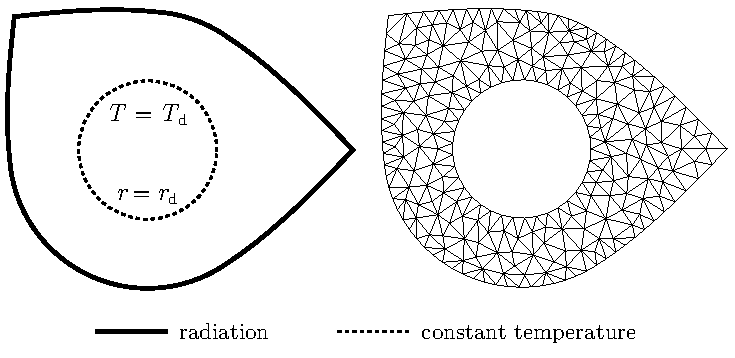
\includegraphics[width=0.8\textwidth]{line-verification-domain-mesh}
  
\includegraphics[width=\textwidth]{line-verification-domain-mesh-legend}
  \caption{
    Selected domain and finite element mesh for numerical verification.
  }
  \label{fig:line-verification-domain-mesh}
\end{figure}

\section{Physical range}
\label{sec:polar.physical}

While it was shown in Section~\ref{sec:polar.convex} that
convex domains can only be constructed
when the dimensionless group~$A$ lies in the interval~%
  (\ref{eq:line-traced-boundary-hot-convex-a-interval}),
there remains yet the practical question of
the physical lengths and temperatures which this translates to.
The results obtained for convex domains
will not be applicable for arbitrary choices
of length and temperature scales,
and in this section we determine the physical range of applicability
corresponding to
the interval~(\ref{eq:line-traced-boundary-hot-convex-a-interval}) in~$A$.

It is appropriate here to return to dimensional variables
by restoring the \scalingmarks{} which have been dropped
from every occurrence of~$\scaled{T}$, $\scaled{r}$, and~$\scaleddel$
starting from~(\ref{eq:line-scaled-radiation-boundary-condition}).

\subsection{Temperature}
\label{sec:polar.physical.temperature}

In a practical situation
one is probably only interested in objects of a given size.
We fix~$r_\sharp$, which is both the physical inradius of any convex domain
constructed in Section~\ref{sec:polar.convex.construction},
and the physical radius of the outer critical terminal curve.
Given the restriction~(\ref{eq:line-traced-boundary-hot-convex-a-interval})
on the possible values of the dimensionless group~$A$,
we would expect a corresponding interval
which restricts the possible values of temperature
\begin{equation}
  T_\sharp = T_0 \log \roundbr*{\frac{r_0}{r_\sharp}}
  \label{eq:line-t-sharp}
\end{equation}
along the incircle~$r = r_\sharp$.

First we observe that
\begin{equation}
  r_0 \ideq \frac{r_\sharp}{\scaled{r}_\sharp},
  \label{eq:line-length-scale-in-terms-of-r-sharp}
\end{equation}
and we recall that
\begin{equation}
  A
  = \psi (\scaled{r}_\sharp)
  = \scaled{r}_\sharp \log^4 \scaled{r}_\sharp
  \label{eq:line-dimensionless-group-in-terms-of-r-sharp}
\end{equation}
from the definition of~$\scaled{r}_\sharp$
(see Item~\ref{itm:polar.regimes.hot}
in Section~\ref{sec:polar.viable.regimes}).
Rearranging~(\ref{eq:line-dimensionless-group})
to give~$T_0$ in terms of~$r_0$ and~$A$,
then substituting~(\ref{eq:line-length-scale-in-terms-of-r-sharp})
and~(\ref{eq:line-dimensionless-group-in-terms-of-r-sharp}),
we obtain
\begin{equation}
  T_0 = \roundbr*{\frac{1}{c r_\sharp \log^4 \scaled{r}_\sharp}}^{1/3}.
  \label{eq:line-temperature-scale-in-terms-of-r-sharp}
\end{equation}
Using this along with~(\ref{eq:line-length-scale-in-terms-of-r-sharp}),
the physical temperature~(\ref{eq:line-t-sharp})
along the incircle~$r = r_\sharp$ becomes
\begin{align*}
  T_\sharp
  &=
    \roundbr*{\frac{1}{c r_\sharp \log^4 \scaled{r}_\sharp}}^{1/3}
    \log \roundbr*{\frac{1}{\scaled{r}_\sharp}}
      \\
  &=
    \roundbr*{\frac{1}{c r_\sharp \log (1 / \scaled{r}_\sharp)}}^{1/3}.
      \yesnumber
      \label{eq:line-t-sharp-in-terms-of-r-sharp}
\end{align*}
Now the interval~(\ref{eq:line-traced-boundary-hot-convex-a-interval}) in~$A$
corresponds to the interval~%
  (\ref{eq:line-traced-boundary-hot-convex-r-sharp-interval})
in~$\scaled{r}_\sharp$,
equivalent to
\begin{equation}
  \frac{1}{4} < \frac{1}{\log (1 / \scaled{r}_\sharp)} \le \frac{1}{2}.
  \label{eq:line-traced-boundary-hot-convex-log-r-sharp-interval}
\end{equation}
Therefore, the physical temperature interval for~$T_\sharp$,
in which convex domains of inradius~$r_\sharp$ can be constructed,
is
\[
  \roundbr*{\frac{1}{4 c r_\sharp}}^{1/3}
    <
  T_\sharp
    \le
  \roundbr*{\frac{1}{2 c r_\sharp}}^{1/3},
\]
or
\begin{equation}
  \roundbr*{\frac{\conduc}{4 \emiss \stefan r_\sharp}}^{1/3}
    <
  T_\sharp
    \le
  \roundbr*{\frac{\conduc}{2 \emiss \stefan r_\sharp}}^{1/3}.
  \label{eq:line-traced-boundary-hot-convex-t-sharp-interval}
\end{equation}
The ratio between the two endpoints is~$\sqrt[3]{2} = 1.2599$.
Note that it is the lower bound which is ultimately important,
since the line-source singularity at~$r = 0$
can always be replaced by a constant-temperature input~$T = T_\dir > T_\sharp$
along some interior circular boundary~$r = r_\dir < r_\sharp$,
where $T_\dir$ and~$r_\dir$ satisfy
\begin{equation}
  T_\dir = T_0 \log \roundbr*{\frac{r_0}{r_\dir}},
  \label{eq:line-equivalent-dirichlet-relation}
\end{equation}
which is the unscaled form
of~(\ref{eq:line-scaled-equivalent-dirichlet-relation}).
For a contrived example,
consider a polyvinyl chloride (PVC) coating
in the shape of a constructed convex domain,
with an effective inradius~$r_\sharp = \SI{4}{\centi\metre}$,
and covering a rod~$r \le r_\dir$
which is held at some constant temperature~$T = T_\dir$.
Using emissivity~$\emiss = 0.93$
and conductivity~$\conduc = \SI{0.18}{\watt \per\metre \per\kelvin}$
for PVC~\cite[Table~2]{lucchi-2018-transient-radiative-rotating-pvc},
the temperature range~%
  (\ref{eq:line-traced-boundary-hot-convex-t-sharp-interval})
evaluates to $\SI{277}{\kelvin} < T_\sharp \le \SI{349}{\kelvin}$,
or~$\SI{4}{\degreeCelsius} < T_\sharp \le \SI{76}{\degreeCelsius}$,
a reasonable interval.

\subsection{Power per unit length}
\label{sec:polar.physical.power}

Although the internal heat generation can be specified
along \emph{any} circle~$r = r_\dir < r_\sharp$,
provided the fixed temperature~$T = T_\dir$
satisfies the condition~(\ref{eq:line-t-sharp}),
the corresponding power per unit length
for all of these choices will be the same,
with the value determined by the strength
of the known line-source solution~(\ref{eq:line-laplace-solution}).
Since the line-source parameters~$T_0$ and~$r_0$ are linked
through the dimensionless constant~$A$,
and since $A$~must lie in the interval~%
  (\ref{eq:line-traced-boundary-hot-convex-a-interval}),
there must be a corresponding interval for the possible values of
power dissipated per unit length.

The line-source solution~(\ref{eq:line-laplace-solution})
has the radial heat flux
\begin{equation}
  -k \del T = \frac{k T_0}{r} \basisvec{r},
  \label{eq:line-heat-flux}
\end{equation}
so that the power per unit length dissipated via conduction
through any closed curve~$r = r (\phi)$
is given by
\begin{equation}
  p =
    \int_{0}^{2 \pi}
      \normalvec \dotp \roundbr[\bulkysize]{-k \del T}
      \cdot r (\phi)
    \td\phi,
  \label{eq:line-power-per-length-closed-curve}
\end{equation}
where $\normalvec$~is the outward unit normal.
Since the only source is the singularity at~$r = 0$ (there are no sinks),
the result of this integral will be the same
along any closed curve containing the origin.
Choosing the interior circular boundary~$r = r_\dir$
for its radial symmetry ($\normalvec = \basisvec{r}$),
we have
\begin{align*}
  p
  &=
    \int_{0}^{2 \pi}
      \basisvec{r} \dotp \frac{k T_0}{r_\dir} \basisvec{r}
      \cdot r_\dir
    \td\phi
      \\[\tallspace]
  &=
    2 \pi k T_0
      \\[\tallspace]
  &=
    2 \pi k
    \roundbr*{\frac{1}{c r_\sharp \log^4 \scaled{r}_\sharp}}^{1/3}
      \yesnumber
      \label{eq:line-power-per-length}
\end{align*}
by~(\ref{eq:line-temperature-scale-in-terms-of-r-sharp}).
Reusing the result~%
  (\ref{eq:line-traced-boundary-hot-convex-log-r-sharp-interval}),
we obtain the desired interval in power per unit length
corresponding to convex domains of inradius~$r_\sharp$:
\[
  2 \pi k \roundbr*{\frac{1}{c r_\sharp} \cdot \frac{1}{4^4}}^{1/3}
    <
  p
    \le
  2 \pi k \roundbr*{\frac{1}{c r_\sharp} \cdot \frac{1}{2^4}}^{1/3},
\]
or
\begin{equation}
  \frac{\pi k^{4/3}}{(32 \emiss \stefan r_\sharp)^{1/3}}
    <
  p
    \le
  \frac{\pi k^{4/3}}{(2 \emiss \stefan r_\sharp)^{1/3}}.
  \label{eq:line-traced-boundary-hot-convex-power-per-length-interval}
\end{equation}
The ratio between the two endpoints is~$2^{4/3} = 2.5198$.
Note that by conservation of energy,
$p$~is also the total power per unit length
lost through the outer boundary via radiation.

Using the parameter values from the PVC example
of Section~\ref{sec:polar.physical.temperature},
the power-per-length interval~%
  (\ref{eq:line-traced-boundary-hot-convex-power-per-length-interval})
evaluates to $\SI{78}{\watt \per\metre} < p \le \SI{198}{\watt \per\metre}$.

\section{Summary}
\label{sec:polar.summary}

In this chapter we have performed boundary tracing
for the conduction--radiation problem in polar coordinates,
starting from the line-source solution~(\ref{eq:line-laplace-solution}).
The geometry of the viable domain depends on the size
of the dimensionless group~(\ref{eq:line-dimensionless-group}),
leading to three regimes qualitywise.
We have shown that convex domains can only be constructed
in the subinterval~(\ref{eq:line-traced-boundary-hot-convex-a-interval})
of the hot regime,
with the radiation boundaries constructed by
making protrusions from the circle~$r = r_\sharp$.
The resulting domains have been validated
by comparing numerical solutions to the conduction--radiation problem
with the exact solution~(\ref{eq:line-laplace-solution}).
Finally, we have determined the physical intervals
for temperature and power per length
which are possible for a given inradius~$r_\sharp$.
